% !TEX root = ../main.tex



\item Drie voorwerpen zijn aan elkaar verbonden met touwtjes. De wrij\-vings\-factor tussen de tafel en het erop liggend voorwerp $V$ is $\mu$.
\begin{figure}[h]
\begin{center}
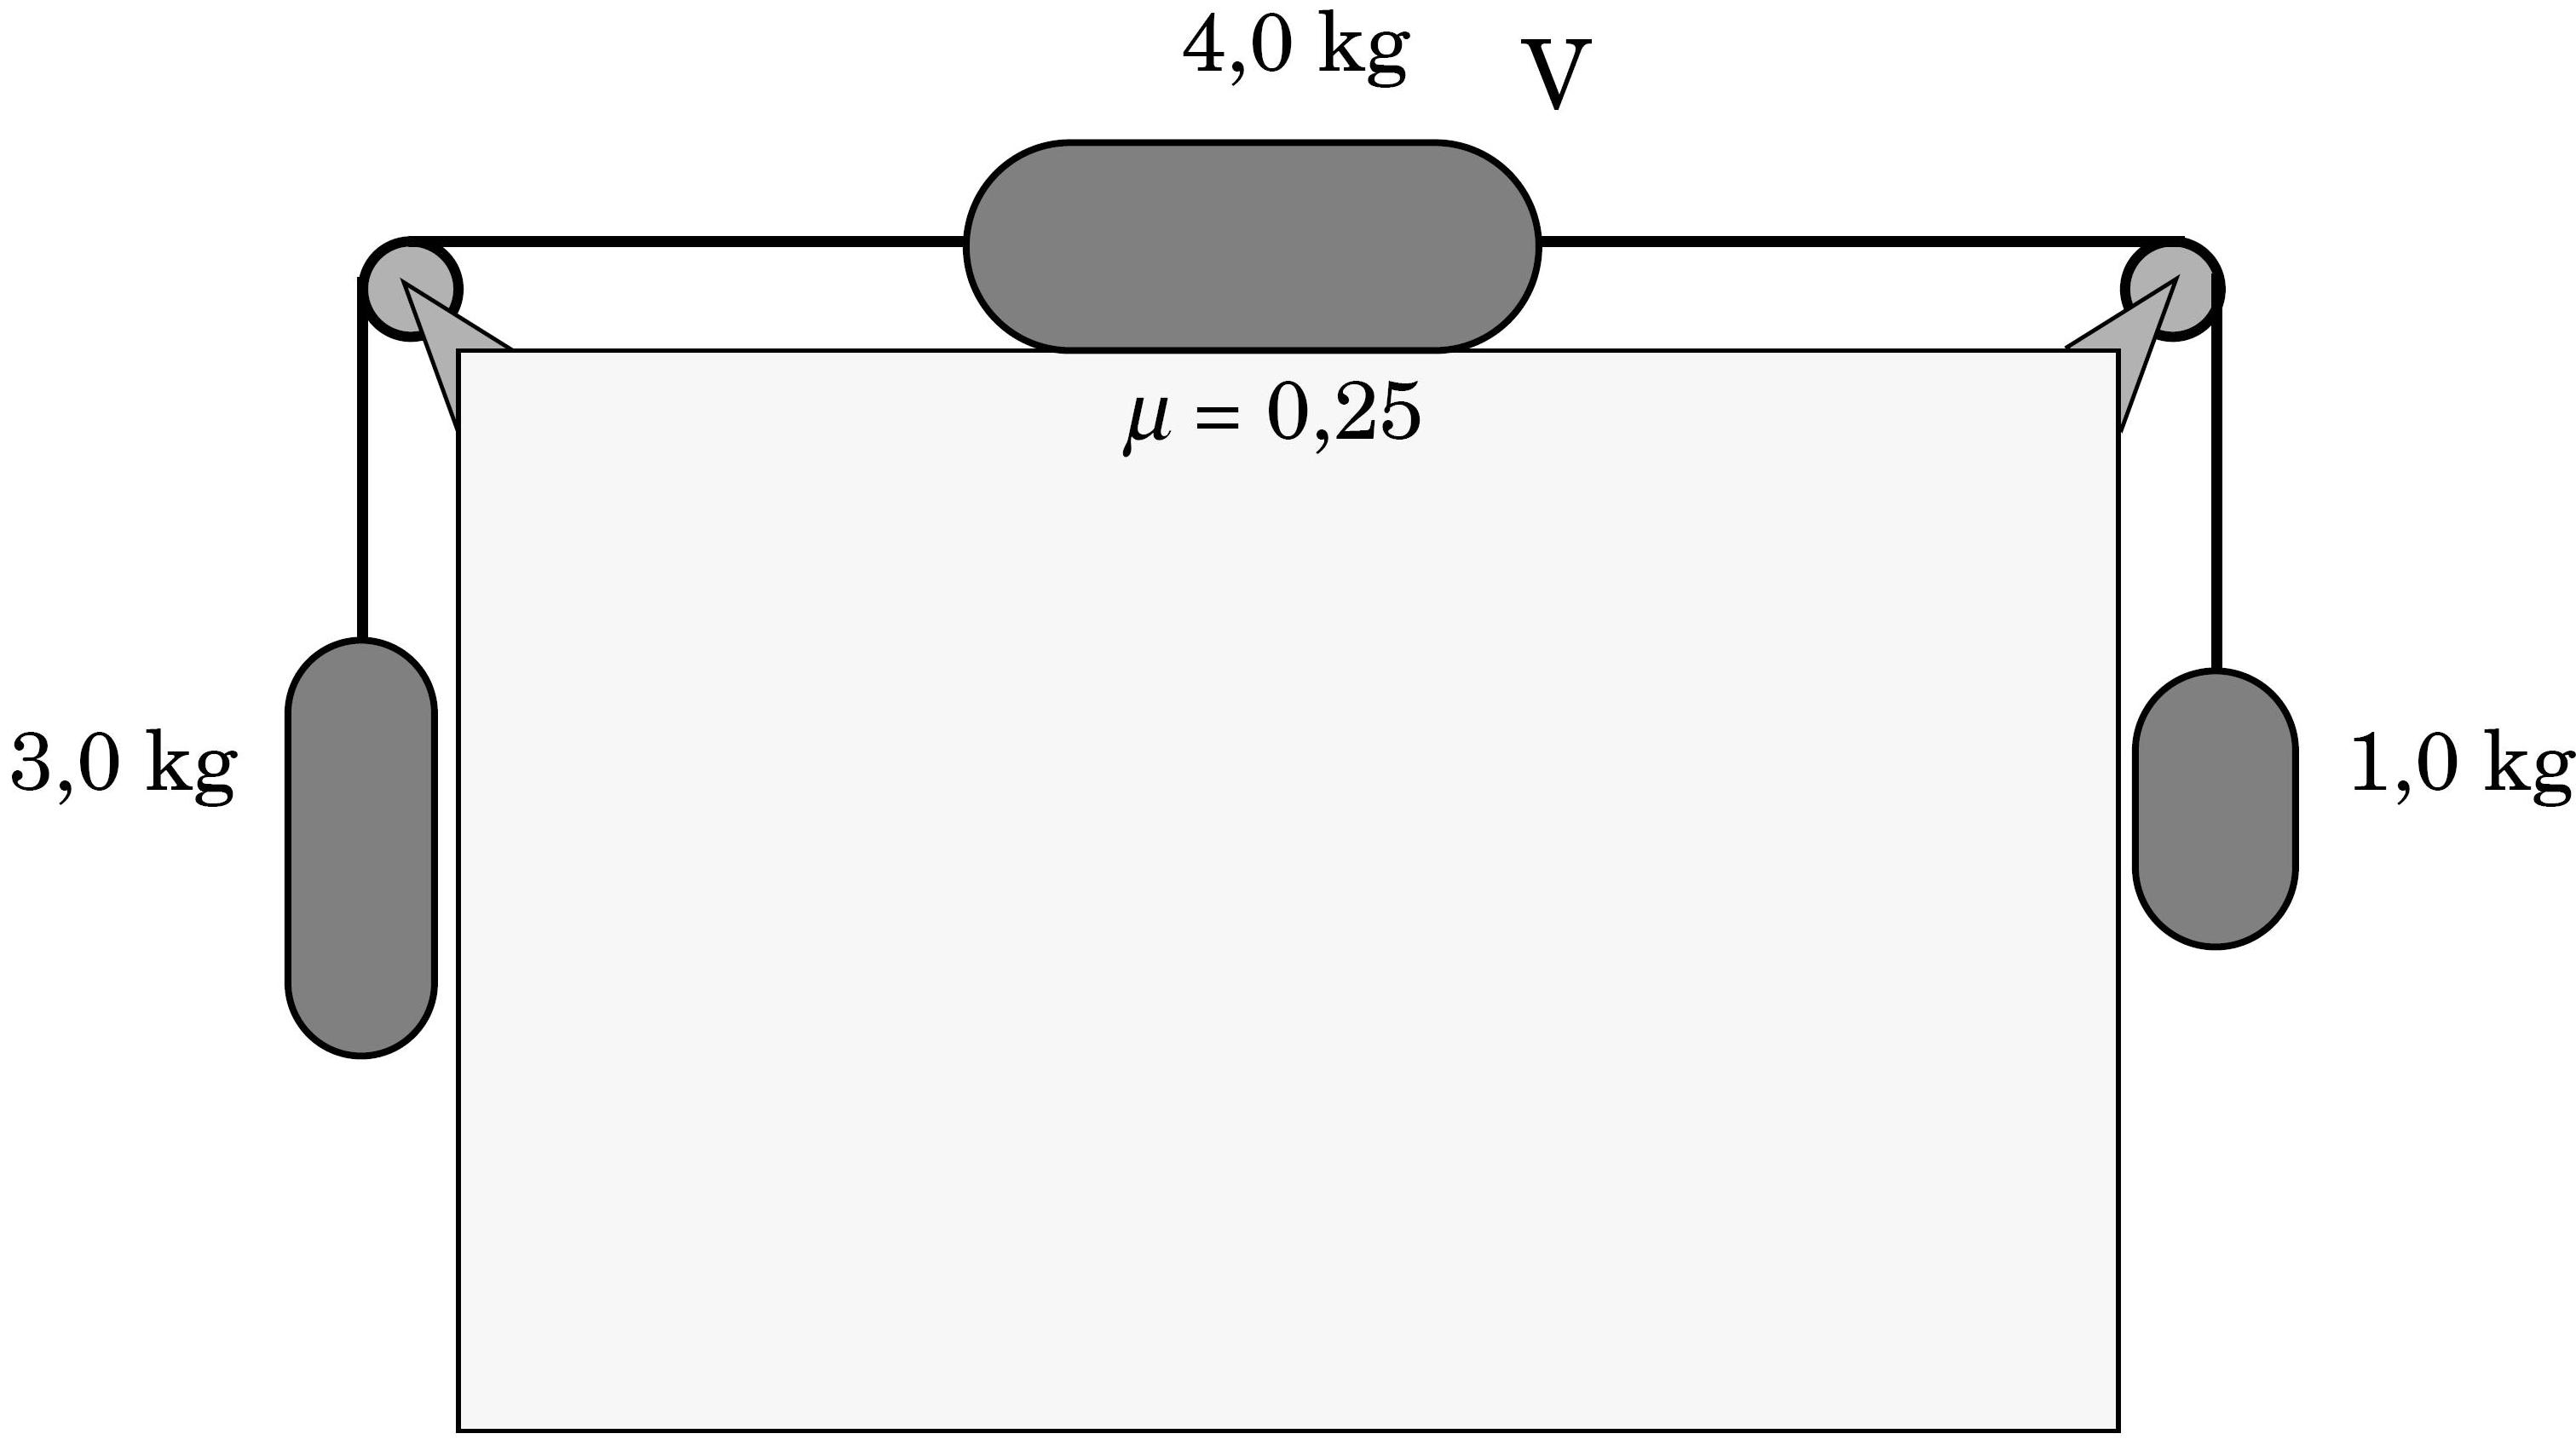
\includegraphics[width=0.6\textwidth ,angle=0]{drie_voorwerpen}
\end{center}
\end{figure}
Veronderstel dat er geen wrijving is in de katrollen en dat de massa van de katrollen te verwaarlozen is. Bepaal de versnelling van het voorwerp. (Bron: 16de VFO 2004)
\begin{oplossing}
\newline
Om de versnelling van het voorwerp te vinden kunnen we de tweede wet van Newton toepassen op de drie massa's. We tekenen de krachtendiagrammen op elk van de massa's (zie figuur). 
\begin{figure}[h]
\begin{center}
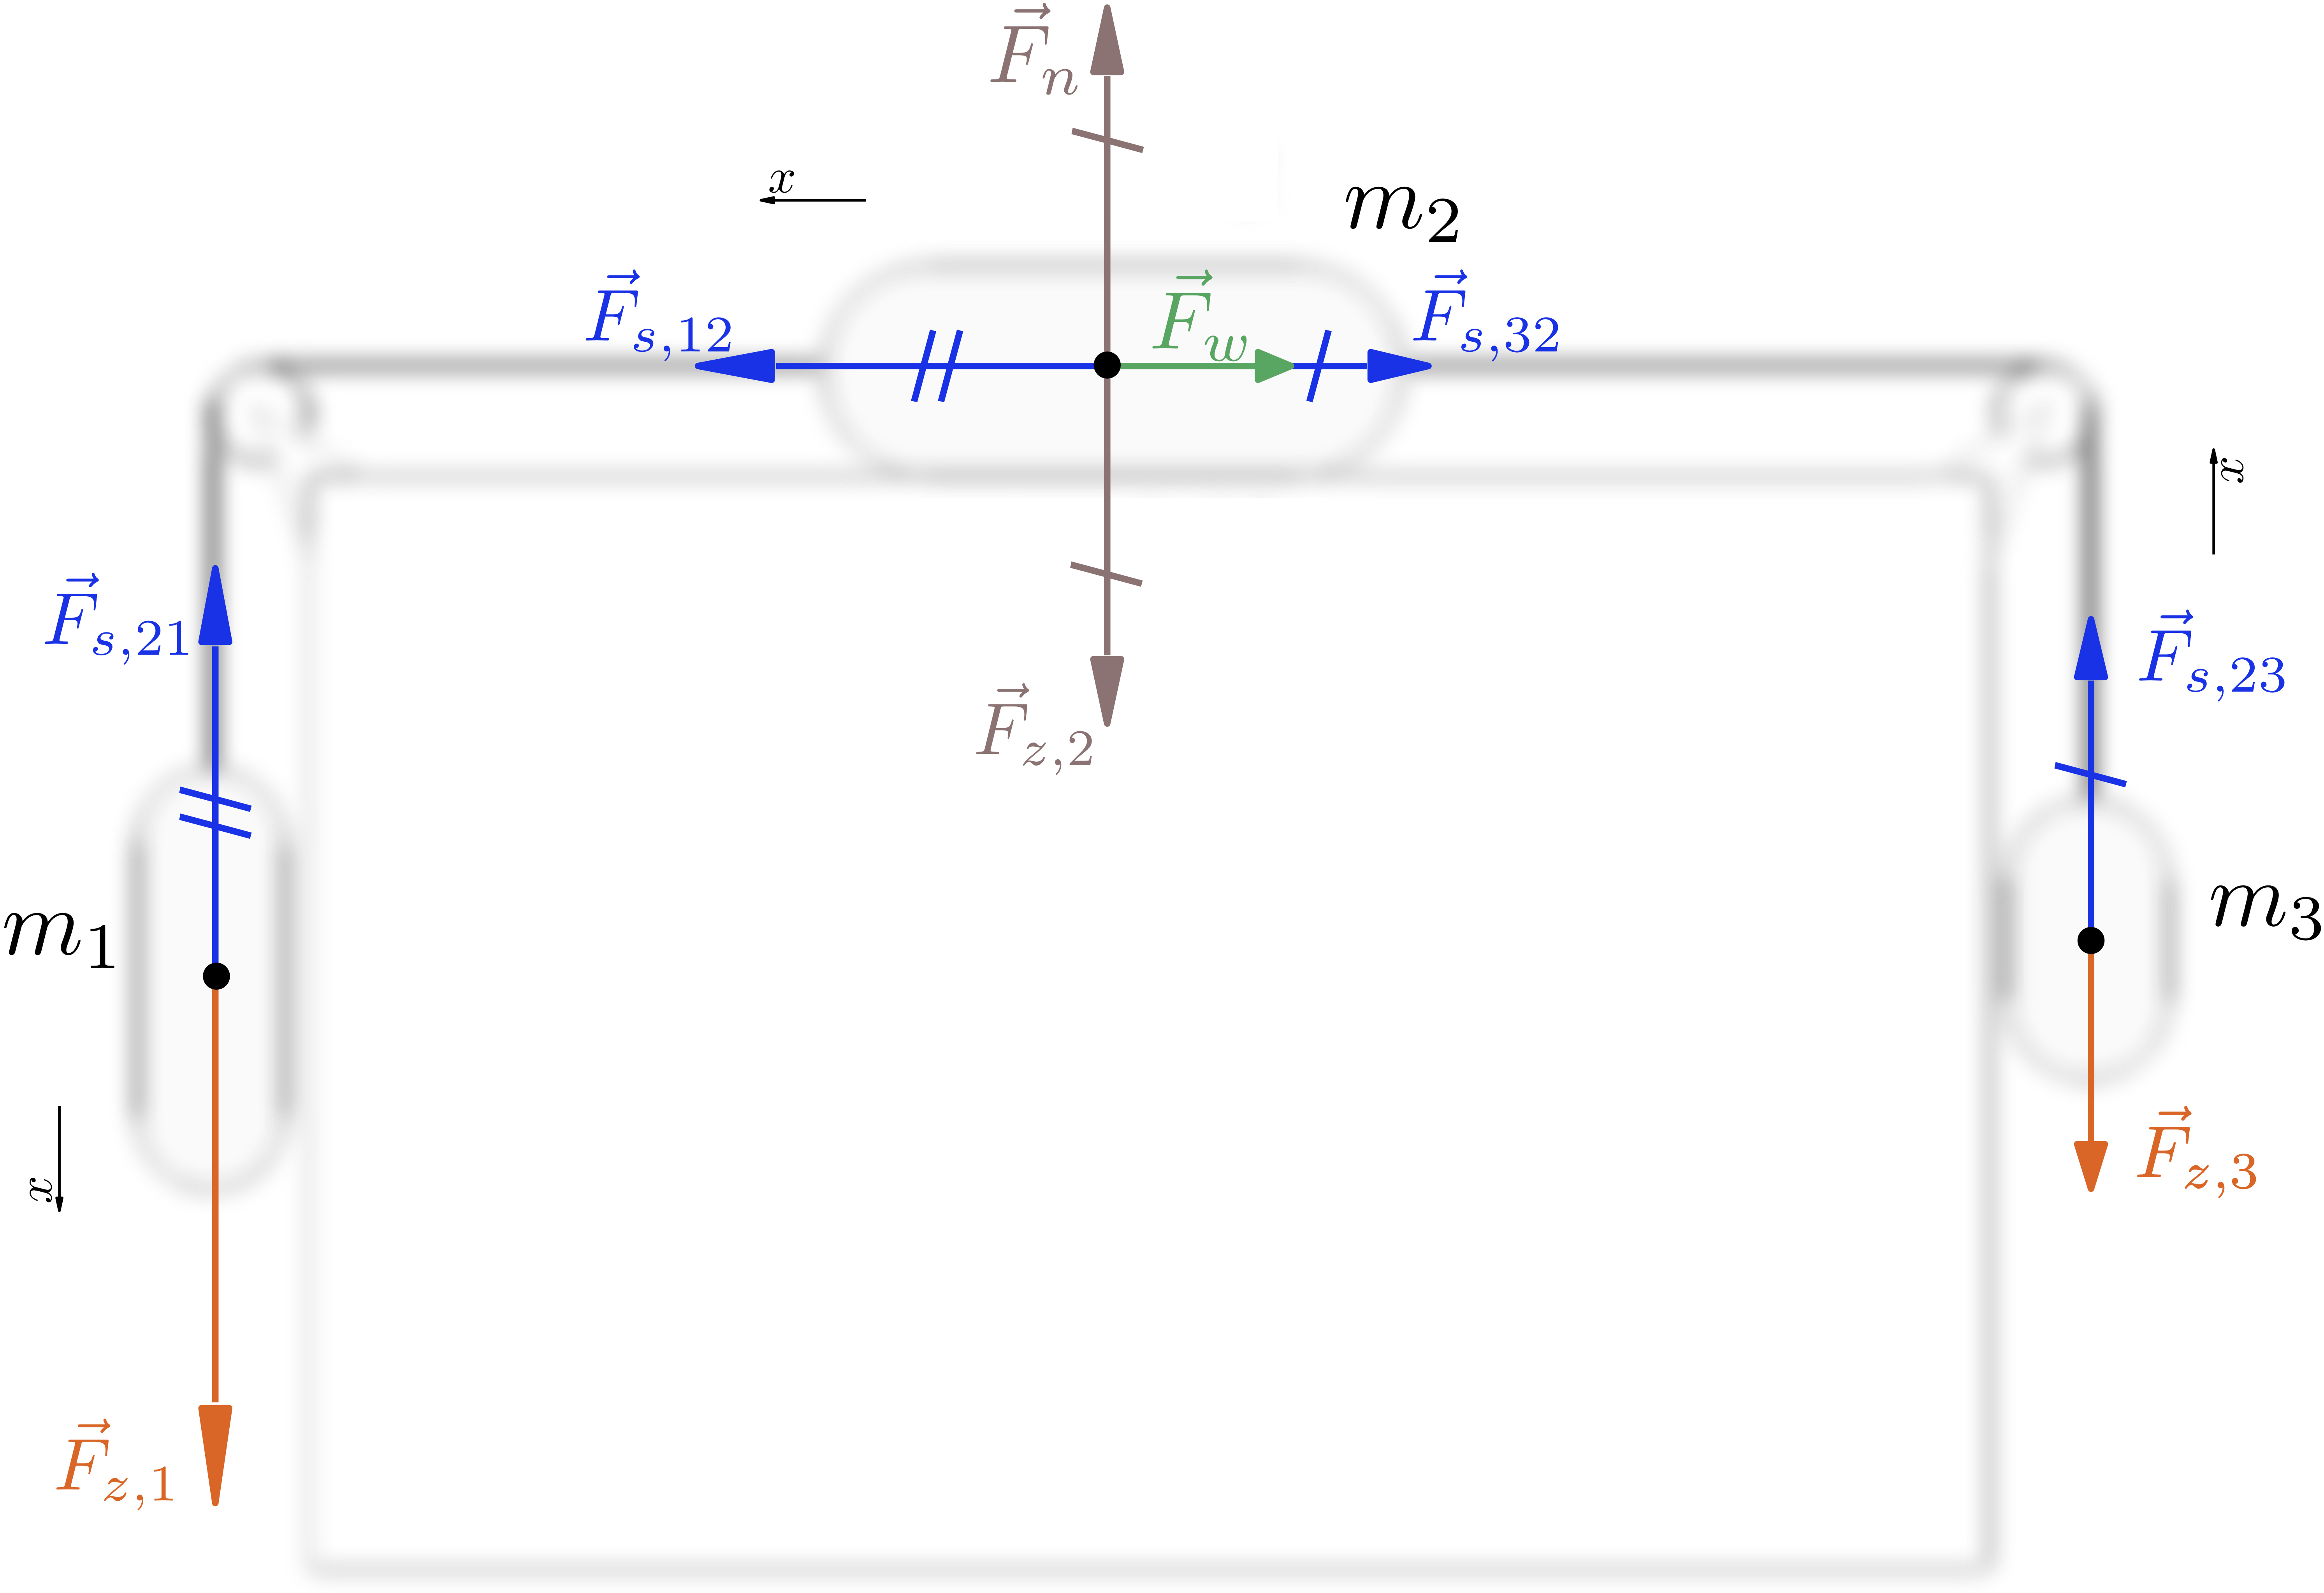
\includegraphics[width=0.73\textwidth ,angle=0]{drie_voorwerpen_krachten}
\end{center}
\end{figure}
\newline
Voor $m_1$ vinden we, met de keuze van de $x$-as verticaal naar beneden:
\begin{eqnarray}
F_{z,1}-F_{s,21}=m_1a\label{m_1}
\end{eqnarray}
Voor $m_3$ vinden we, met nu de keuze van de $x$-as verticaal naar boven:
\begin{eqnarray}
F_{s,23}-F_{z,3}=m_3a\label{m_3}
\end{eqnarray}
Voor $m_2$ vinden we, met de keuze van de $x$-as horizontaal naar links:
\begin{eqnarray}
F_{s,12}-F_w-F_{s,32}=m_2a\label{m_2}
\end{eqnarray}
Volgens de derde wet van Newton kunnen we de overeenkomstige spankrachten aan mekaar gelijk stellen: $F_{s,21}=F_{s,12}$ en $F_{s,32}=F_{s,23}$. Samen met $F_w=\mu F_n$ en $F_z=ma$ hebben we drie vergelijkingen en drie onbekenden. Oplossen naar de versnelling levert:
\begin{eqnarray*}
a=\frac{m_1-m_2-\mu m_3}{m_1+m_2+m_3}g=1,2\rm\,m/s^2
\end{eqnarray*}
\newline
\newline
Realiseer je dat de keuze van de $x$-as bij het bepalen van de componenten van de krachten de tekens bepalen van die componenten -- en ook die van de versnelling. Als je bijvoorbeeld tweemaal $a$ schrijft (in vergelijking (\ref{m_1}) en (\ref{m_3})) moet het ook effectief over dezelfde versnelling gaan, en niet over versnellingen die elkaars tegengestelde zijn. Met de $x$-as verticaal naar beneden geori\"enteerd voor $m_1$, zal de versnelling voor $m_1$ positief zijn als de massa naar beneden versnelt (wat hij doet; $m_1>m_3$). Voor $m_3$ moet je dan de $x$-as verticaal omhoog kiezen, wil je dat $a$ evenzeer positief is of dus dezelfde betekenis heeft.
\newline
\newline
Zie ook dat uit vergelijking (\ref{m_1}) volgt dat $m_1$ niet met de zwaartekracht aan $m_2$ trekt! De massa $m_1$ versnelt, waarvoor een resulterende kracht nodig is. 
\end{oplossing}